\section{User Interfaces}

% \begin{subbox}{Tasks}
%     \begin{enumerate}
%         \item Create a storyboard for the application - it can be a ppt or even a video. Embed the ppt/video in the pdf submission of this week.
%         \item Take each user story and create low-fidelity wireframes
%         \item Apply usability design guidelines and heuristics discussed in lectures to come up with the wireframes.
%     \end{enumerate}
% \end{subbox}

\subsection{Storyboards}
Based on the user stories, 4 boards have been identified to summarise functionality of the app:
\begin{enumerate}
    \tightlist
    \item Student Storyboard (\autoref{fig:stu_sb})
    \item Admin Storyboard (\autoref{fig:admin_sb})
    \item Course Team Member Storyboard (\autoref{fig:ctm_sb})
    \item IITM Management Storyboard (\autoref{fig:im_sb})
\end{enumerate}

\begin{figure}[H]
    \centering
    \fbox{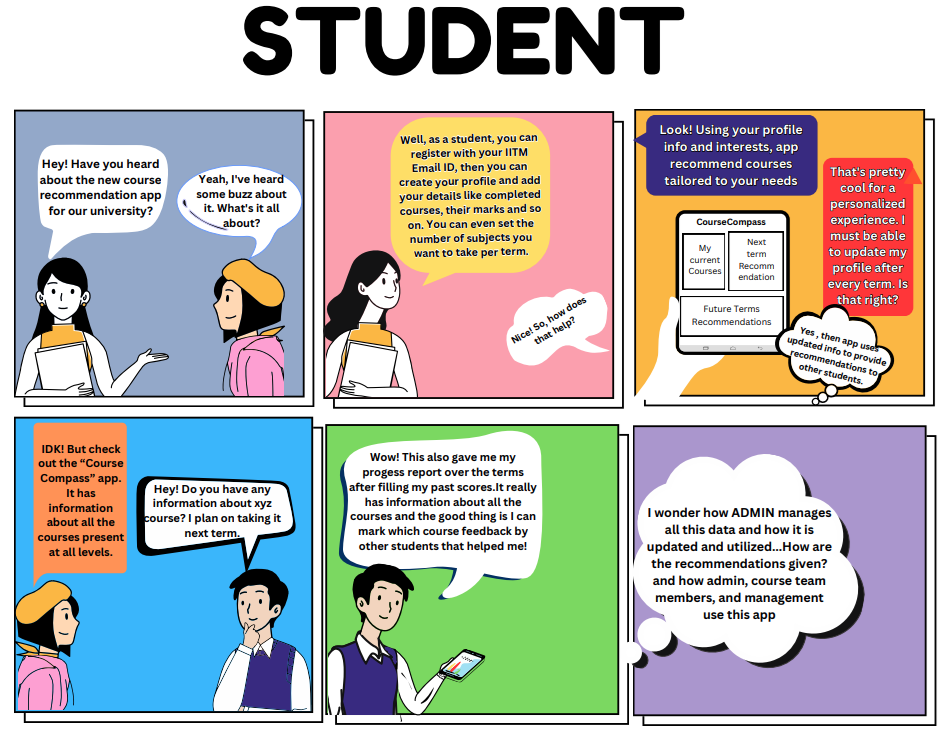
\includegraphics[width=1\textwidth]{img/sb1.png}}
    \caption{Student Storyboard}
    \label{fig:stu_sb}
\end{figure}
\begin{figure}[H]
    \centering
    \fbox{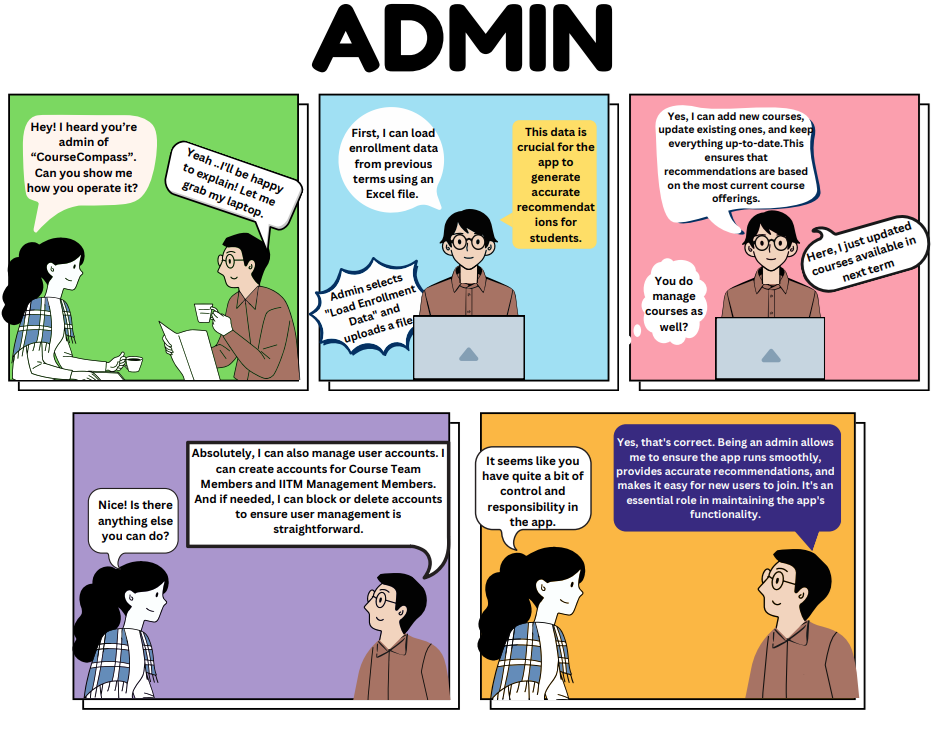
\includegraphics[width=0.875\textwidth]{img/sb2.png}}
    \caption{Admin Storyboard}
    \label{fig:admin_sb}
\end{figure}
\begin{figure}[H]
    \centering
    \fbox{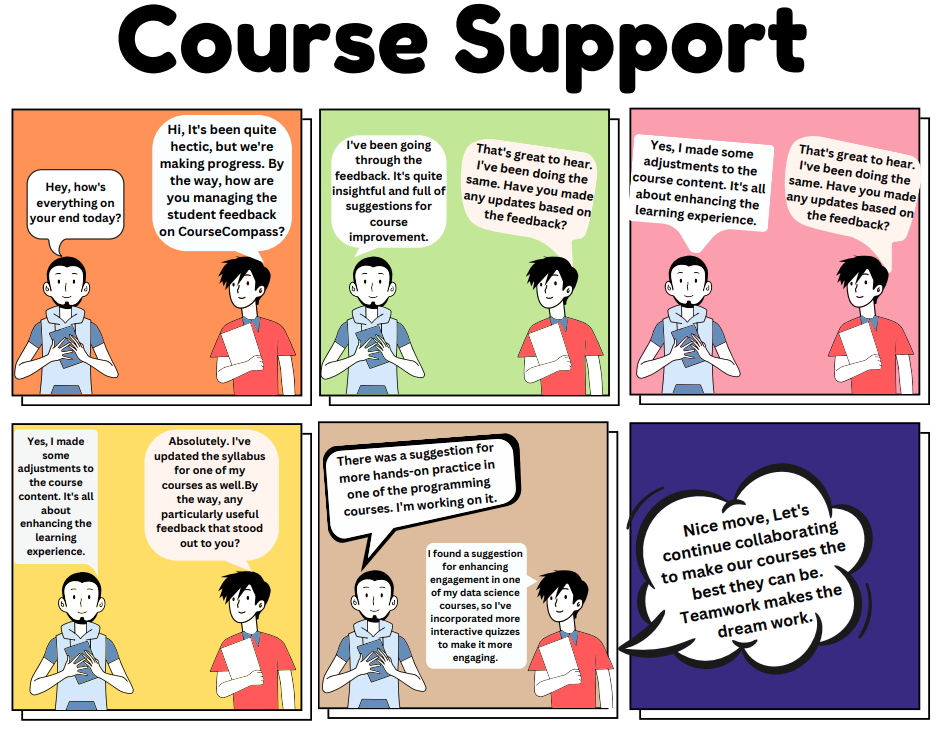
\includegraphics[width=0.875\textwidth]{img/sb3.png}}    \caption{Course Team Member Storyboard}
    \label{fig:ctm_sb}
\end{figure}
\begin{figure}[H]
    \centering
    \fbox{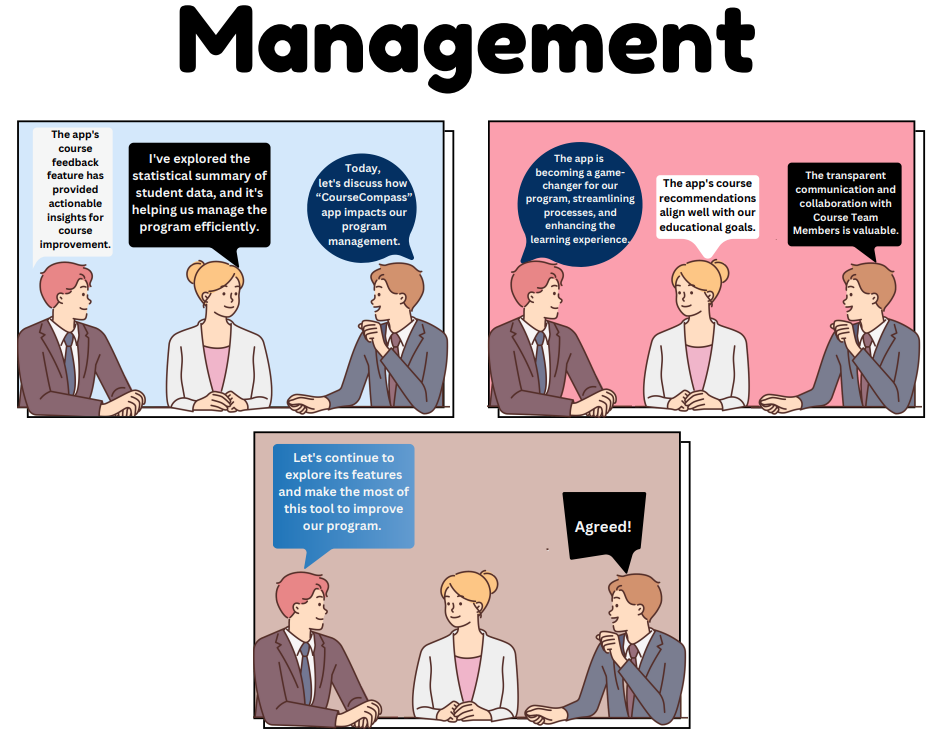
\includegraphics[width=1\textwidth]{img/sb4.png}}
    \caption{IITM Management Storyboard}
    \label{fig:im_sb}
\end{figure}

\subsection{Wireframes}
Based on these storyboards and user stories, the following unique pages have been identified to be created:
\begin{enumerate}
    \tightlist
    \item Login/Registration Page (\autoref{fig:login})
    \item Student's Homepage (\autoref{fig:stu_home})
    \item Student's Profile page (\autoref{fig:stu_profile})
    \item A Page for Students to view all the courses (\autoref{fig:stu_allcourses})
    \item A page for Student to view individual course its feedback (\autoref{fig:stu_course_feedback})
    \item Administrator dashboard (\autoref{fig:admin_dash})
    \item A page enlisting all courses to the Administrator (\autoref{fig:admin_all_courses})
    \item A page to add/edit courses for the Administrator (\autoref{fig:admin_add_edit_course})
    \item A page for administrator that enlists course team members, IITM management members and other admins (\autoref{fig:admin_entity_page})
    \item A page for Adding / Editing course team members, IITM management members and other admins (\autoref{fig:admin_ae_entity})
    \item Course team members’ Dashboard (\autoref{fig:ctm_dash})
    \item A page for Course Team Members to view feedback given by students (\autoref{fig:ctm_feedback})
    \item A page for Course team members for adding / updating course description (\autoref{fig:ctm_ae_description})
    \item IITM Management Dashboard (similar to \autoref{fig:admin_dash})
    \item IITM Management Course Feedback page (\autoref{fig:im_courses})
\end{enumerate}

\subsubsection{General Wireframes}
\begin{figure}[H]
    \centering
    \fbox{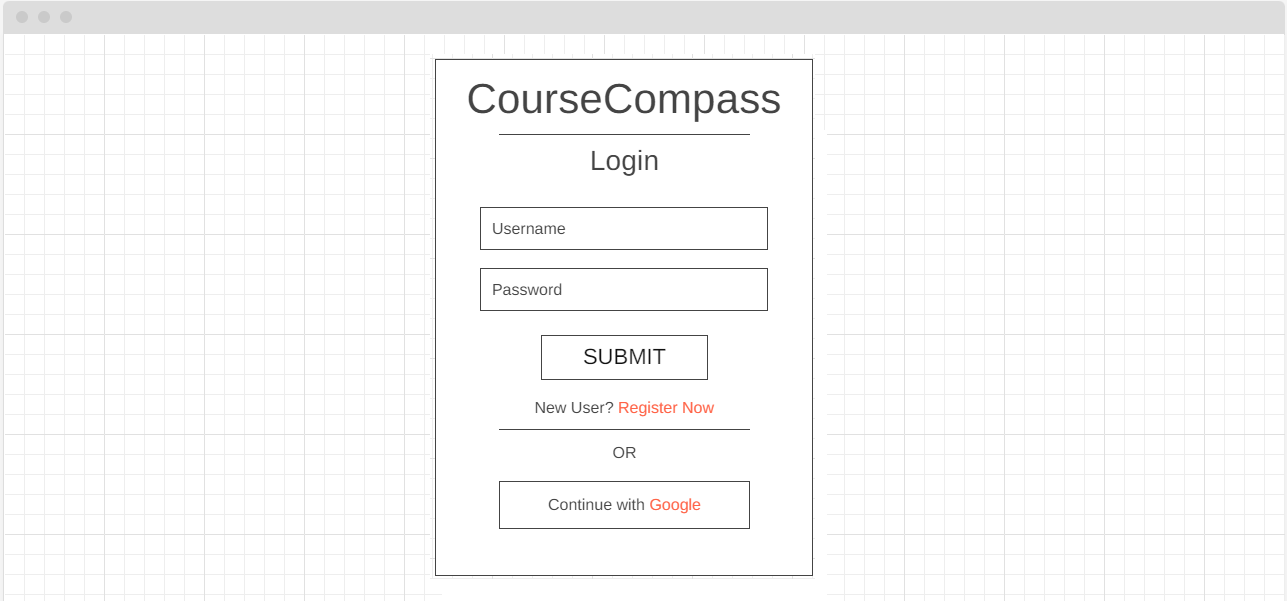
\includegraphics[width=1\textwidth]{img/1.LandingPage.png}}
    \caption{Login Page (Registration page will also look similar)}
    \label{fig:login}
\end{figure}

\subsubsection{Students Pages' Wireframes}
\begin{figure}[H]
    \centering
    \fbox{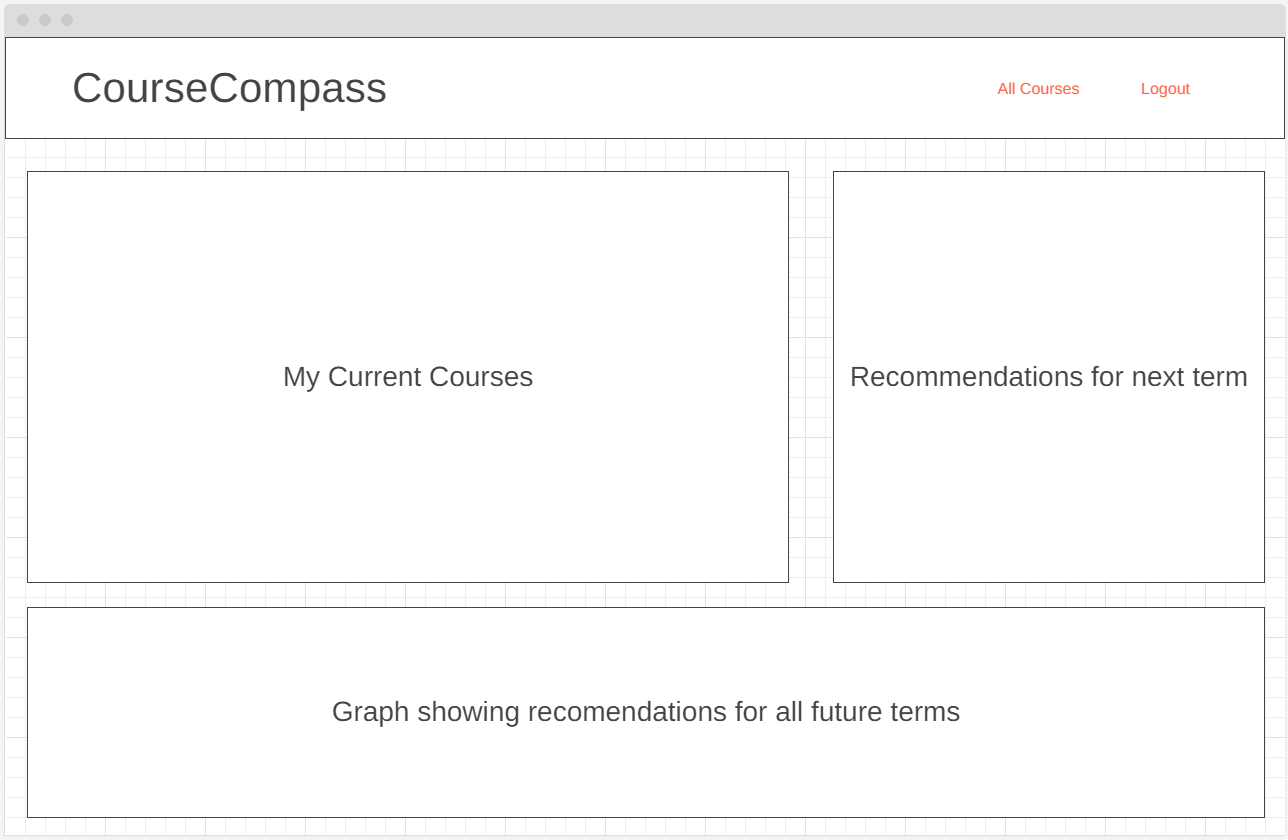
\includegraphics[width=1\textwidth]{img/2.stuHome.png}}
    \caption{Student's homepage}
    \label{fig:stu_home}
\end{figure}

\begin{figure}[H]
    \centering
    \fbox{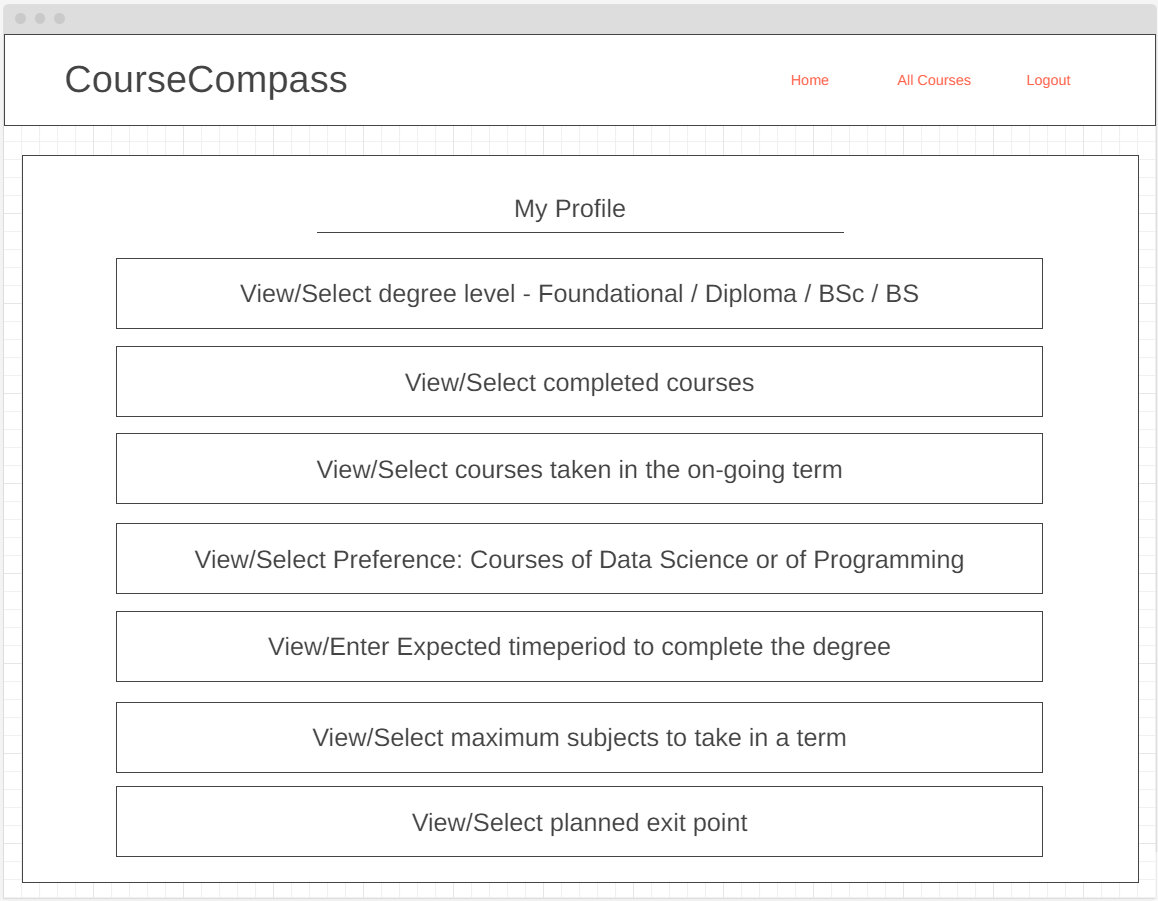
\includegraphics[width=1\textwidth]{img/3.stu_profile.png}}
    \caption{Student's profile page}
    \label{fig:stu_profile}
\end{figure}

\begin{figure}[H]
    \centering
    \fbox{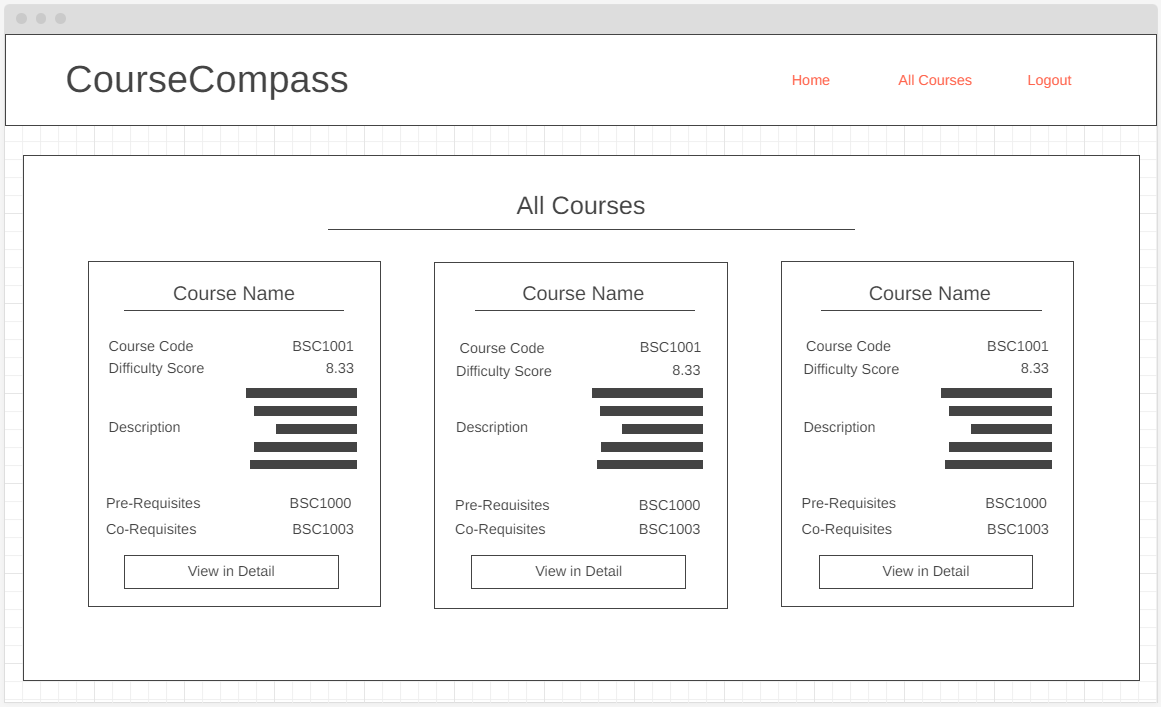
\includegraphics[width=1\textwidth]{img/4.stu_allcourses.png}}
    \caption{Page for Students to view all the courses}
    \label{fig:stu_allcourses}
\end{figure}

\begin{figure}[H]
    \centering
    \fbox{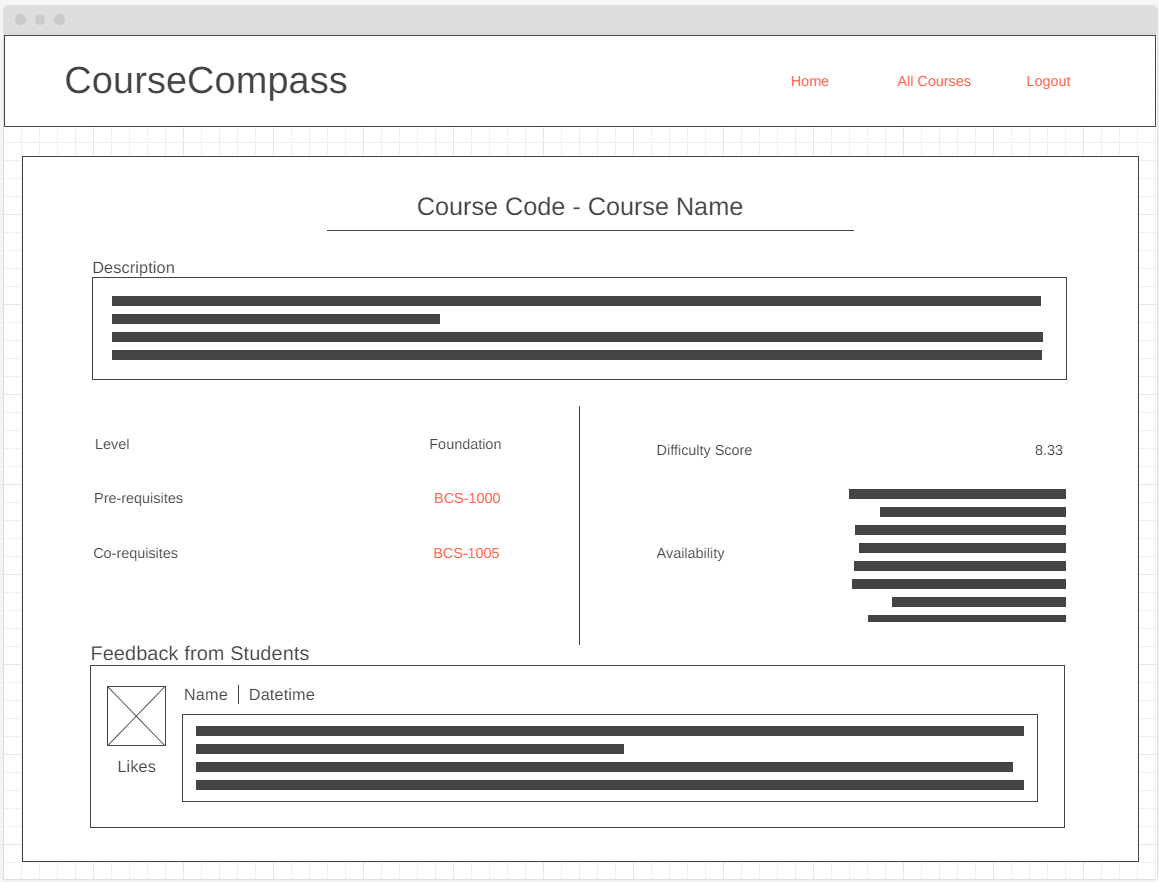
\includegraphics[width=1\textwidth]{img/5.stu_course.png}}
    \caption{Student's courses and feedback page}
    \label{fig:stu_course_feedback}
\end{figure}


\subsubsection{Administrators Pages' Wireframes}
\begin{figure}[H]
    \centering
    \fbox{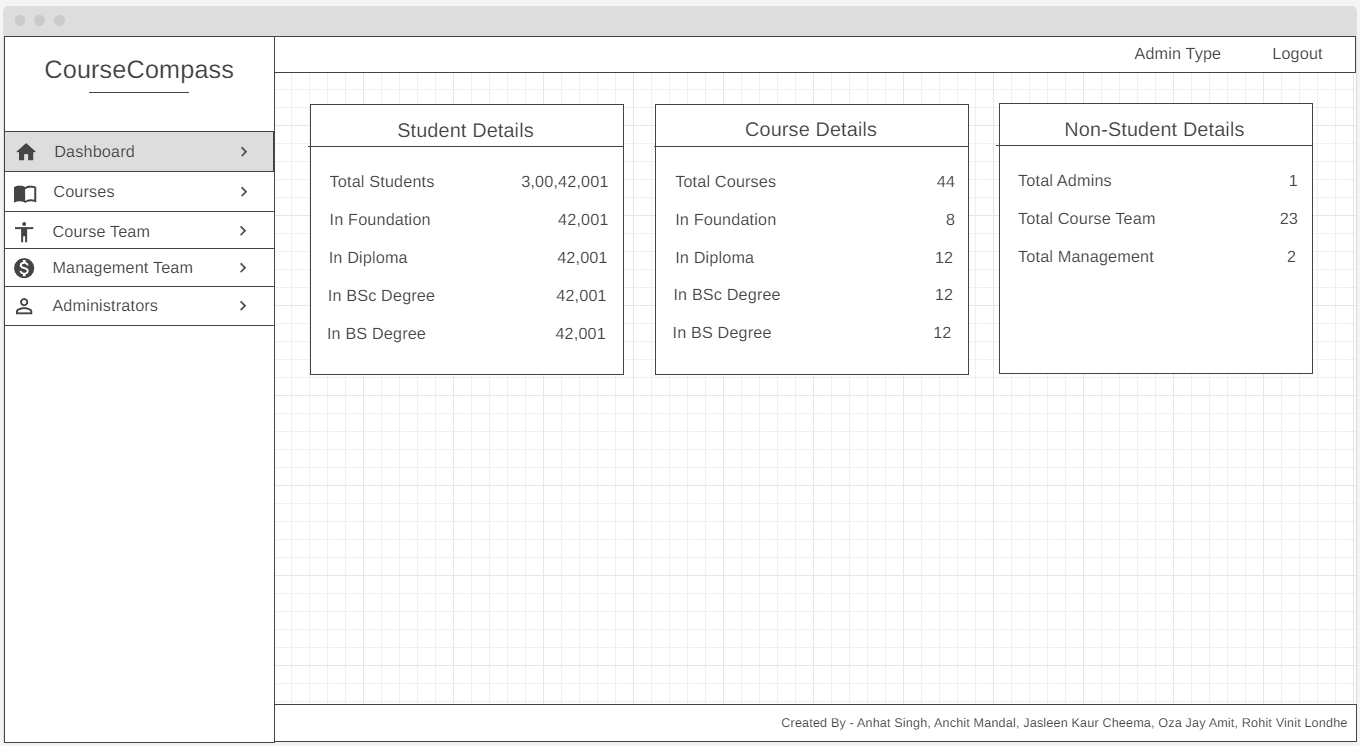
\includegraphics[width=1\textwidth]{img/6.admin_dashboard.png}}
    \caption{Administrator dashboard}
    \label{fig:admin_dash}
\end{figure}

\begin{figure}[H]
    \centering
    \fbox{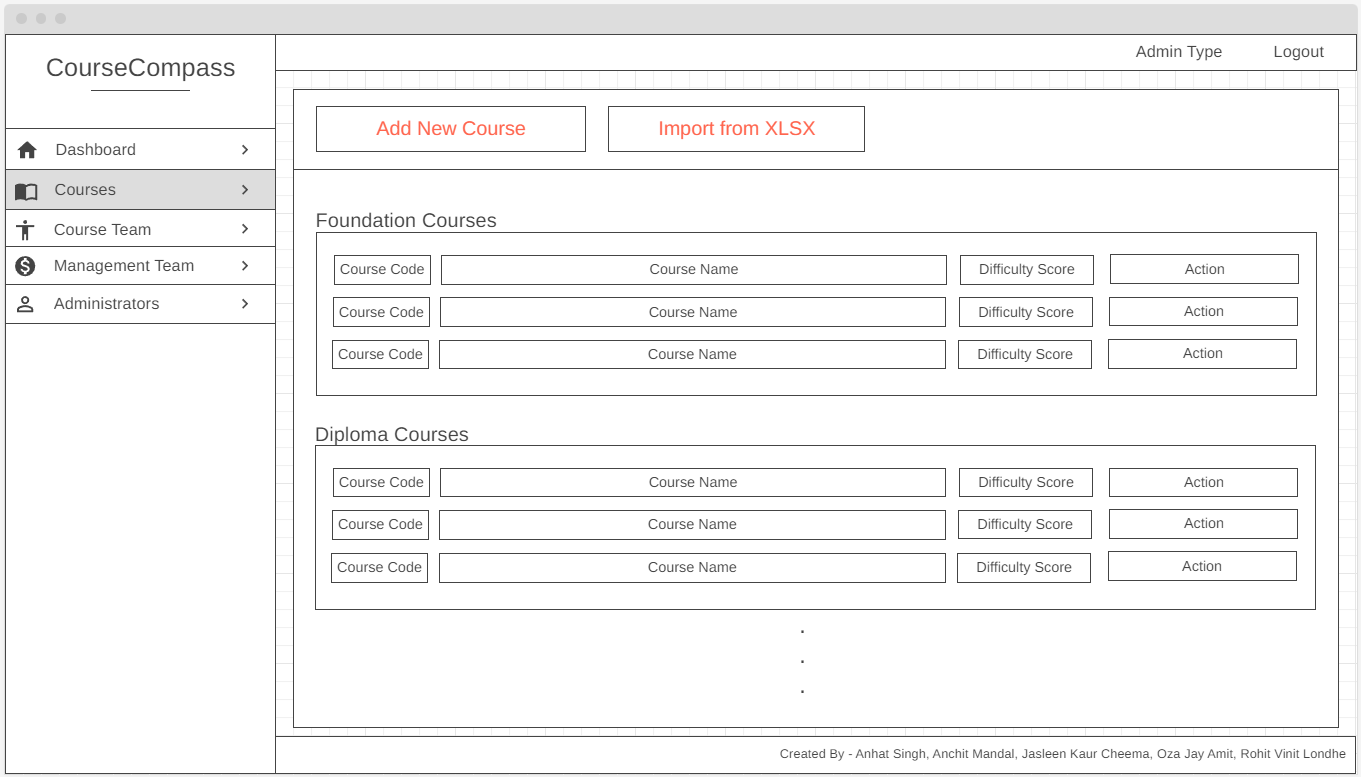
\includegraphics[width=1\textwidth]{img/7.admin_allcourses.png}}
    \caption{Administrator all courses page}
    \label{fig:admin_all_courses}
\end{figure}

\begin{figure}[H]
    \centering
    \fbox{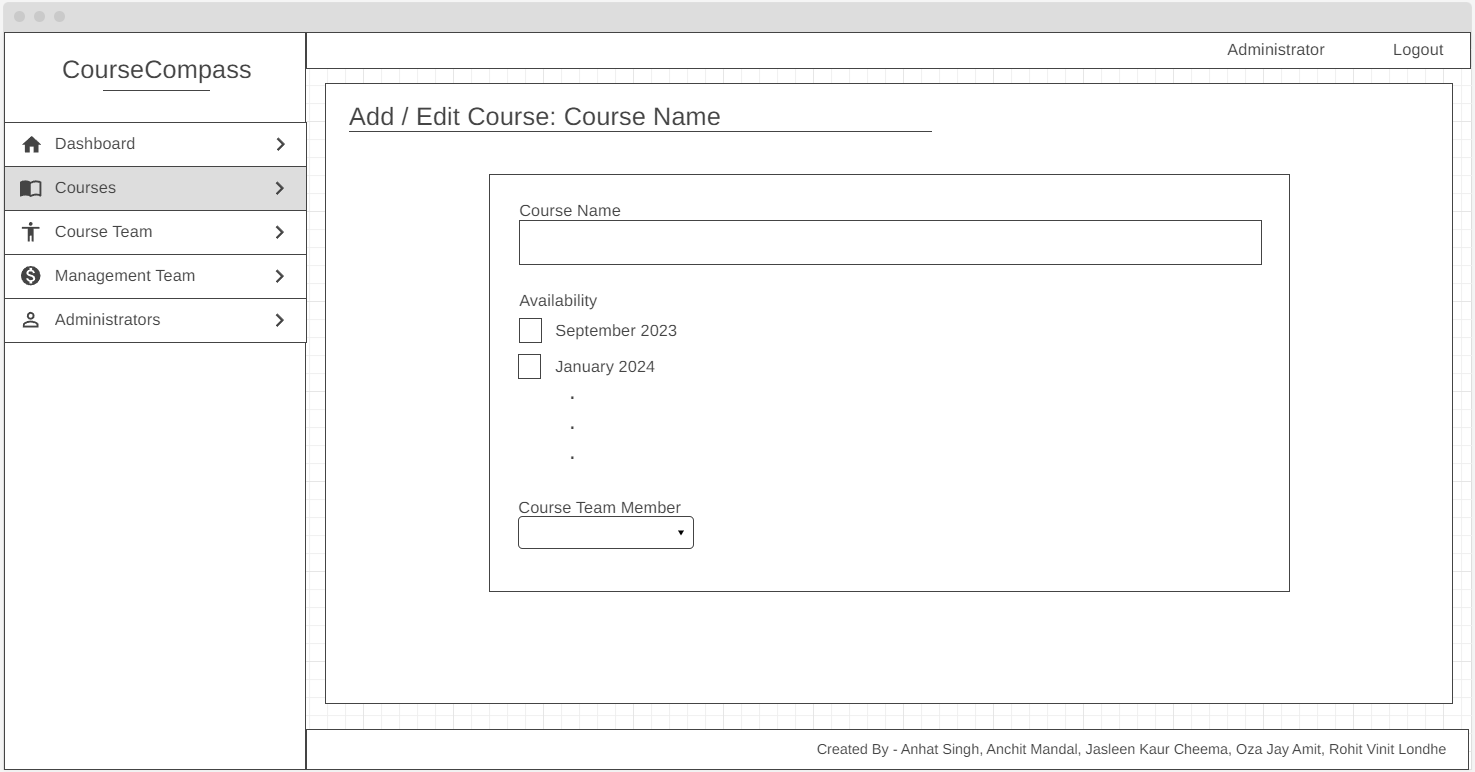
\includegraphics[width=1\textwidth]{img/8.admin_ae_course.png}}
    \caption{Administrator add / edit courses page}
    \label{fig:admin_add_edit_course}
\end{figure}

\begin{figure}[H]
    \centering
    \fbox{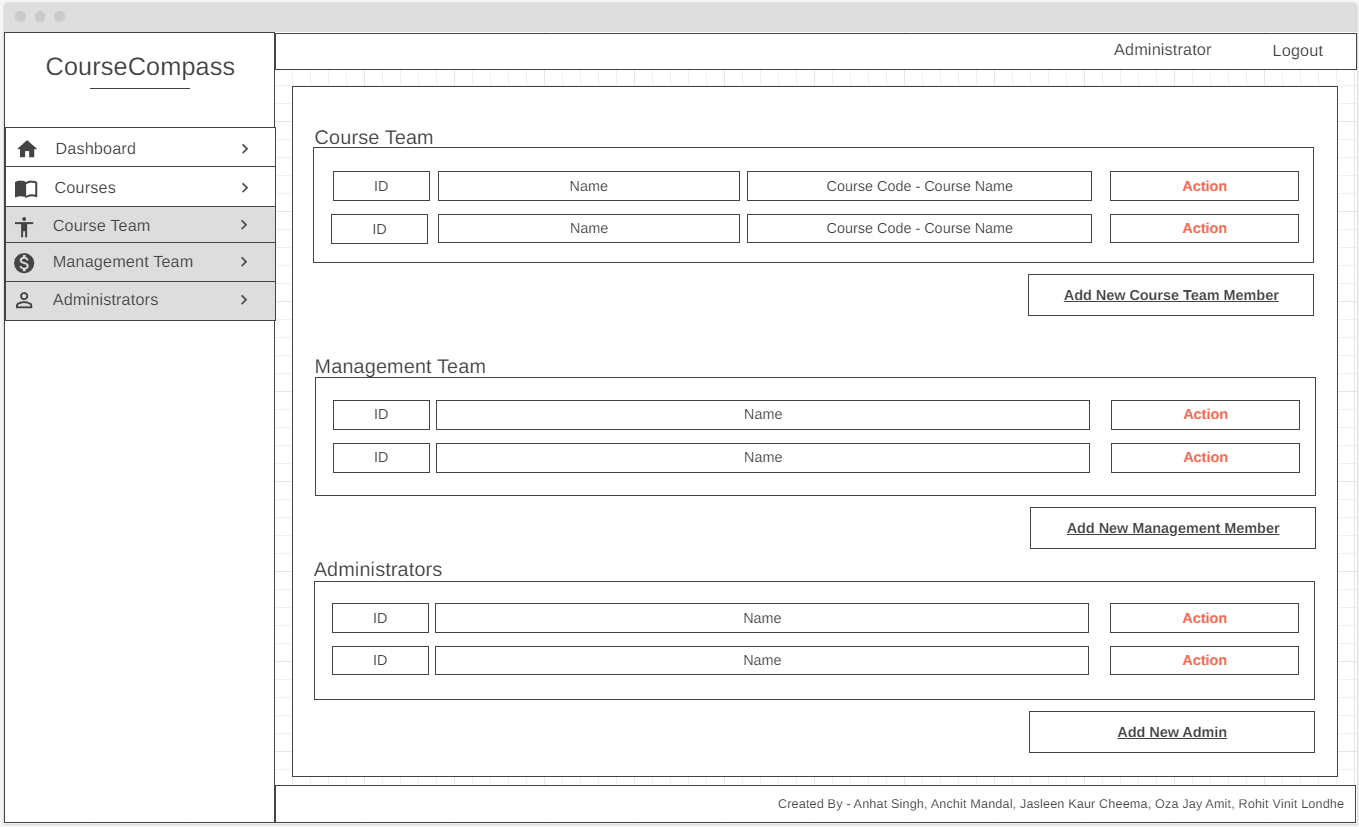
\includegraphics[width=1\textwidth]{img/9.admin_entity_list.png}}
    \caption{Administrator Page to view course team members, IITM management members and other admins}
    \label{fig:admin_entity_page}
\end{figure}

\begin{figure}[H]
    \centering
    \fbox{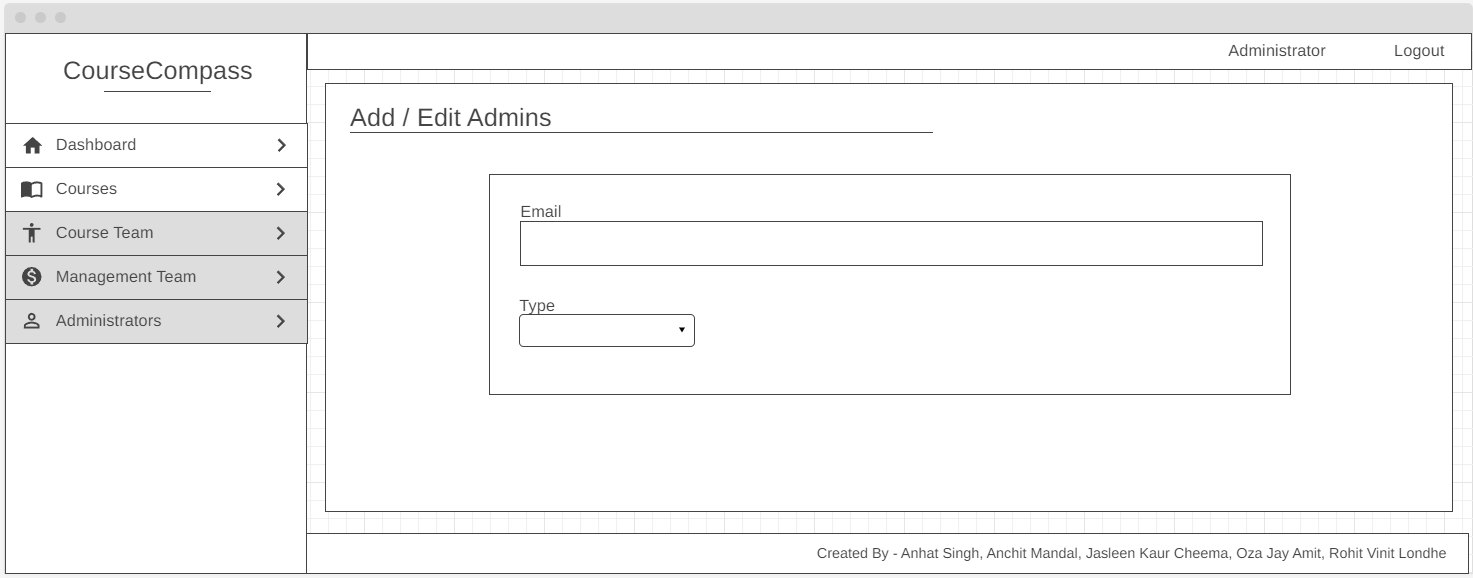
\includegraphics[width=1\textwidth]{img/10.admin_ae_entity.png}}
    \caption{Adding / Editing course team members, IITM management members and other admins}
    \label{fig:admin_ae_entity}
\end{figure}


\subsubsection{Course Team Member Pages' Wireframes}
\begin{figure}[H]
    \centering
    \fbox{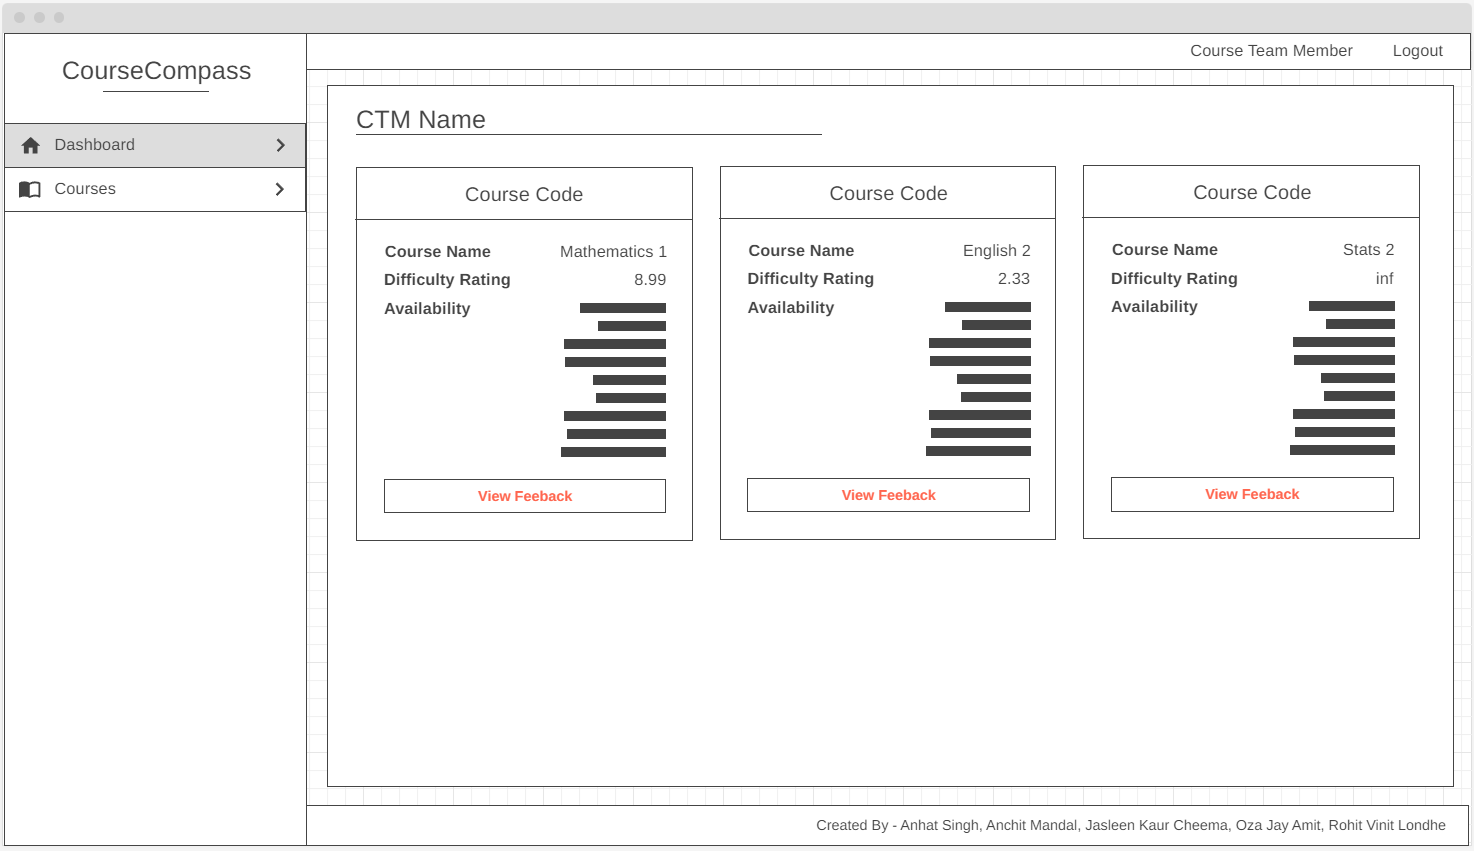
\includegraphics[width=1\textwidth]{img/11.ctm_courses.png}}
    \caption{Course team members' Dashboard}
    \label{fig:ctm_dash}
\end{figure}

\begin{figure}[H]
    \centering
    \fbox{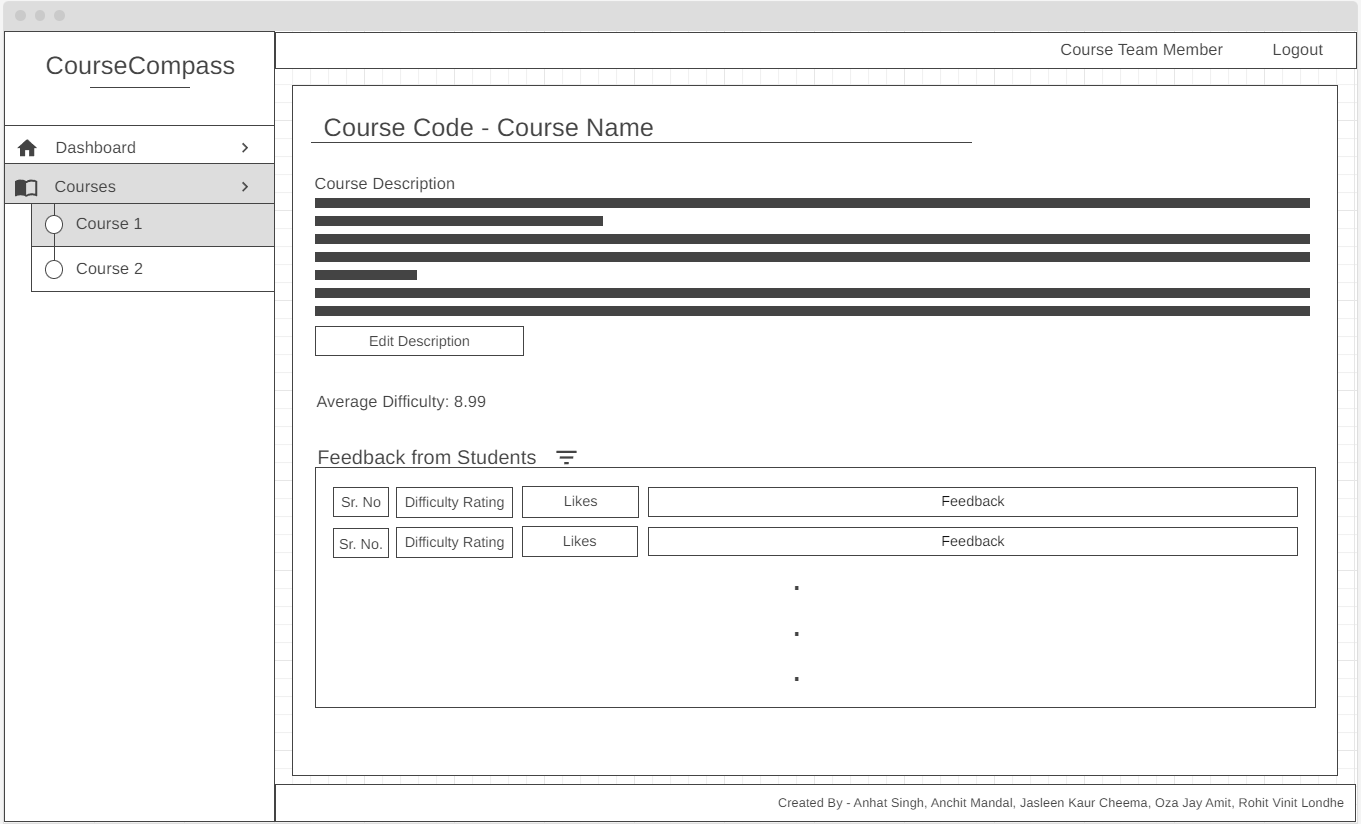
\includegraphics[width=1\textwidth]{img/12.ctm_feedback.png}}
    \caption{A page for Course Team Members to view feedback given by students}
    \label{fig:ctm_feedback}
\end{figure}

\begin{figure}[H]
    \centering
    \fbox{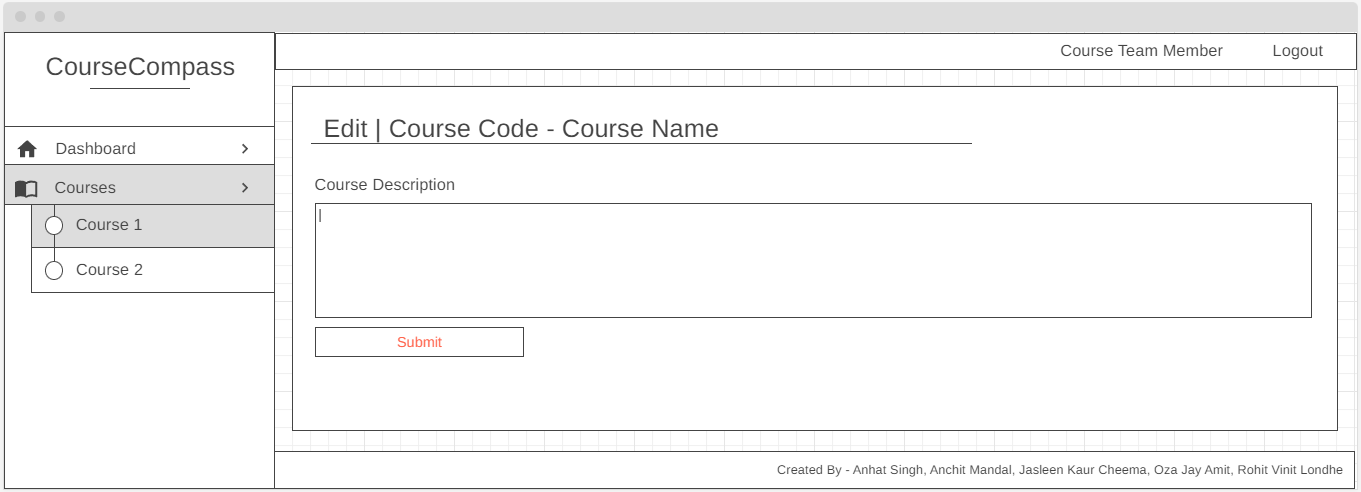
\includegraphics[width=1\textwidth]{img/13.ctm_desc.png}}
    \caption{A page for Course team members for adding / updating course description}
    \label{fig:ctm_ae_description}
\end{figure}


\subsubsection{IITM Management Pages' Wireframes}
\begin{figure}[H]
    \centering
    \fbox{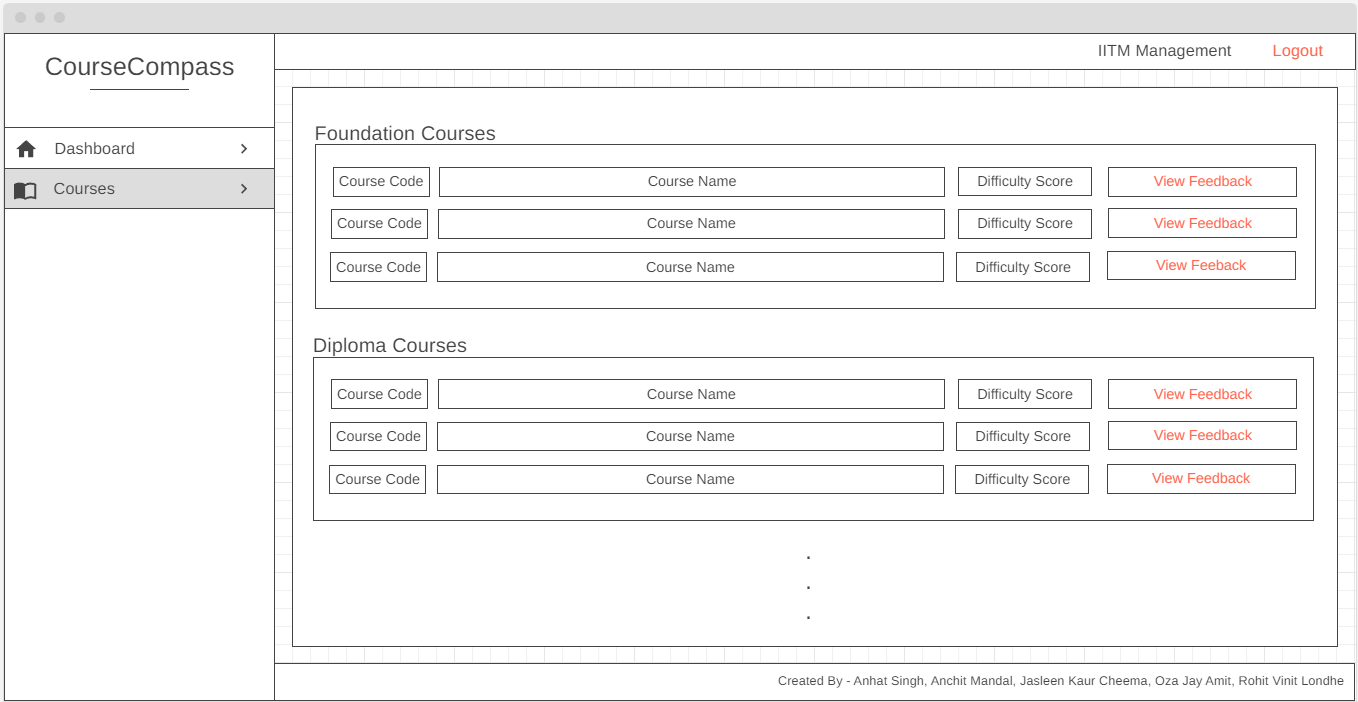
\includegraphics[width=1\textwidth]{img/15.im_allcourses.png}}
    \caption{IITM Management Course Feedback page}
    \label{fig:im_courses}
\end{figure}


\subsection{Usability Design Guidelines \& Heuristics}
The low-fidelity wireframes have been designed with common Design guidelines (Effectivess, Effeciency, Safety, Learnability, Memorability) ensuring that it is obvious what each page displays and easy to determine the flow of information. Here are some specific recommendations based on these principles followed while creating the wireframes:

\begin{enumerate}
    \item \textbf{Registration and Profile Creation}
        \begin{itemize}
            \tightlist
            \item \textbf{Efficiency}: Make the registration process straightforward and efficient. Use email verification for account creation.
            \item \textbf{Memorability}: Ensure that users can easily update their profiles after registration. Use a clear and accessible interface.
        \end{itemize}
    \item \textbf{Interest Selection}
        \begin{itemize}
            \tightlist
            \item \textbf{Effectiveness}: Make it easy for students to select their primary interests. Provide clear options for Data Science, Programming, or Both.
            \item \textbf{Memorability}: Allow users to change their primary interests later if needed.
        \end{itemize}
        
    \item \textbf{Recommendations}
        \begin{itemize}
            \tightlist
            \item \textbf{Effectiveness}: Display recommendations based on a student's profile clearly and prominently.
        \end{itemize}


\item \textbf{Course Information}
    \begin{itemize}
        \tightlist
        \item \textbf{Effectiveness}: Provide detailed course information, including prerequisites, feedback, and difficulty ratings.
        \item \textbf{Memorability}: Use a consistent layout for displaying course details and feedback.
    \end{itemize}


\item \textbf{Admin Features}
    \begin{itemize}
        \tightlist
        \item \textbf{Efficiency}: Admin features should be accessible from a centralized dashboard. Ensure quick data loading from Excel files and easy course management.
        \item \textbf{Safety}: Implement authentication and authorization for admin functions to prevent unauthorized access or modifications.
    \end{itemize}

\item \textbf{Course Team and Management Access}
    \begin{itemize}
        \tightlist
        \item \textbf{Effectiveness}: Ensure that Course Team Members and IITM Management can access student feedback and statistics efficiently.
        \item \textbf{Usability}: Provide user-friendly interfaces for adding, updating, and viewing course details and feedback.
    \end{itemize}


\item \textbf{Statistical Summaries}
    \begin{itemize}
        \tightlist
        \item \textbf{Effectiveness}: Display academic and student data summaries in a clear and informative manner for both students and management.
        \item \textbf{Memorability}: Use consistent visual representations for statistics.
    \end{itemize}


\item \textbf{Feedback Interaction}
    \begin{itemize}
        \tightlist
        \item \textbf{Efficiency}: Allow students, Course Team Members, and IITM Management to interact with feedback efficiently, such as +1 (upvoting) helpful feedback.
        \item \textbf{Usability}: Implement clear feedback forms and voting mechanisms.
    \end{itemize}

\item \textbf{Consistency}
    \begin{itemize}
        \tightlist
        \item \textbf{Usability}: Maintain a consistent design throughout the application to ensure users can easily navigate and understand the interface.
    \end{itemize}

\item \textbf{User Assistance and Help}
    \begin{itemize}
        \tightlist
        \item \textbf{Usability}: Provide tooltips, help sections, or a knowledge base to assist users in understanding how to use the software effectively and safely.
    \end{itemize}


\item \textbf{Error Handling}
    \begin{itemize}
        \tightlist
        \item \textbf{Safety}: Implement user-friendly error messages and validation checks to prevent user errors and ensure safe operation.
    \end{itemize}


\item \textbf{Responsive Design}
    \begin{itemize}
        \tightlist
        \item \textbf{Usability}: Ensure that the UI is responsive and works well on various devices and screen sizes to cater to a broader user base.
    \end{itemize}


\item \textbf{Testing and Feedback}
    \begin{itemize}
        \tightlist
        \item \textbf{Effectiveness}: Regularly test the UI with actual users and collect their feedback to make continuous improvements in line with user needs and preferences.
    \end{itemize}

\end{enumerate}